\chapter{State of the art}
\label{ch:stand-van-zaken}

% Tip: Begin elk hoofdstuk met een paragraaf inleiding die beschrijft hoe
% dit hoofdstuk past binnen het geheel van de bachelorproef. Geef in het
% bijzonder aan wat de link is met het vorige en volgende hoofdstuk.

% Pas na deze inleidende paragraaf komt de eerste sectiehoofding.

Het is al geen geheim meer dat AR op het web zijn intrede doet in de technologiewereld. Er zijn tal van opportuniteiten en manieren waar de juiste bedrijven hun slag mee kunnen slaan. Maar wat komt hier allemaal bij kijken en hoe kan zo'n bedrijf hiermee aan de slag gaan? 

In dit hoofdstuk wordt er verder gegaan op de huidige stand van zaken omtrent AR op het web. Hoe werkt AR precies? Welke types AR zijn er? Moet ik als bedrijf mij op een bepaald type apparaat focussen? Zoja, op welk type? Wat is het verschil tussen ARCore van Google en ARKit Apple? Wat zijn vervolgens de mogelijkheden wanneer ik als bedrijf een AR-ervaring wil creëren voor gebruikers op een iOS apparaat en wat zijn de mogelijkheden wanneer ik dat wil doen op een apparaat zoals Android? Zijn er ook andere opties?

\section{Types AR}
\label{sec:types-ar}
Wanneer een gebruiker wil interageren met een gegenereerde wereld zijn er eerst nog enkele vragen die de AR applicatie moet beantwoorden. Wat moet er precies getoond worden in de gegenereerde wereld en waar moet het getoond worden? Hoe deze vragen beantwoord worden hangt af van het type van de AR applicatie. ~\textcite{Paladini2018} haalt aan dat er drie types AR zijn. 

\textbf{Markerbased AR}

In sommige gevallen moet de applicatie weten naar wat hij kijkt. Dit wordt marker based AR genoemd. De applicatie heeft dan een merkteken nodig in de echte wereld om vervolgens hier de digitale wereld op te tonen. Zo'n merkteken is vaak een prent met bijvoorbeeld het logo van een bedrijf erop. Eenmaal de applicatie dit merkteken via de camera herkent, kan het bijvoorbeeld ook zien dat het punt gedraaid is en dus ook het object draaien en er op plaatsen. Er staan online enkele handleidingen hoe het mogelijk is marker based AR te implementeren in een website. Een voorbeeld hiervan is te volgen in het artikel \textcite{Etienne2017}. Hier wordt er uitgelegd hoe een ontwikkelaar aan zijn eigen website een marker based AR functie kan toevoegen, hiervan het model dat getoond wordt op het merkteken kan veranderen en het merkteken waarop het model staat kan veranderen.

\textbf{Markerless AR}

In een andere situatie is zo'n referentiepunt echter niet nodig en wordt de ruimte rond de gebruiker gescand om te wereld te kunnen herkennen en hier vervolgens objecten in te visualiseren. Hierbij wordt er gesproken over markerless AR. Een voorbeeld hiervan is de IKEA Place app waarbij u zonder merkteken het meubelstuk in de omgeving rond u kan plaatsen en vervolgens kan bewegen naar de geschikte plaats.

\textbf{Location based AR}
Bij het derde type moet de applicatie de gebruiker zijn locatie weten. Dit type noemt men location based AR. Hierbij wordt er AR-informatie gelinkt aan uw locatie. Indien u dan bijvoorbeeld naast een gebouw staat waarvan er AR-informatie bestaat zoals de naam, kan deze informatie geprojecteerd worden op dat gebouw. 



\section{Google ARCore vs Apple ARKit}
\label{sec:google-arcore-vs-apple-arkit}

Google en Apple zijn twee extreem grote bedrijven die heel veel investeren in de race om de beste AR-visualisatie te bieden op smartphones die natuurlijk hun besturingssysteem draaien. Beiden hebben een AR-ontwikkelingsplatform gecreëerd die in grote lijnen gelijk zijn maar toch op sommige vlakken zich van elkaar onderscheiden. Bij Google is dit ARCore en bij Apple is dit ARKit. Kiezen met welk platform er aan de slag wordt gegaan is dus een heel belangrijke stap. 

\subsection{Gemeenschappelijke features}

De meest essentiële features in AR zoals light estimation, environmental understanding en motion tracking zijn bij beide concurrenten uiteraard geïmplementeerd maar hebben hier en daar toch wat verschillen. 

\textbf{Light Estimation}

Beeld u eens in dat u met uw smartphone in een donkere ruimte bent. Uw helderheid wordt waarschijnlijk op een lagere stand gezet. Dit gebeurt aan de hand van de lichtsensoren die in uw smartphone zitten. Deze sensoren meten de omgeving en nemen een gemiddelde om vervolgens daarmee uw helderheid in te stellen. In AR wordt diezelfde technologie gebruikt om de lichtinval op het gevisualiseerde object te verlichten. Zodanig dat indien u bijvoorbeeld buiten bent, het object er verlicht uit zal zien.

\textbf{Environmental understanding}

Environmental understanding is het proces voor het zien, verwerken en gebruiken van zichtbare informatie in de omgeving van het apparaat. Hierbij gaat het apparaat horizontale en verticale vlakten (planes) gaan detecteren zodat het vervolgens daarop de 3D-objecten kan plaatsen.

\textbf{Motion tracking}

Motion tracking zorgt er voor dat wanneer er bewogen wordt met het apparaat, terwijl er al een object in de omgeving geprojecteerd wordt, het object stil blijft staan en u een soepele ervaring beleeft. Op die manier kan u als gebruiker bijvoorbeeld in uw kamer rondwandelen om een geprojecteerd meubelstuk te bekijken vanuit alle perspectieven. Het proces dat dit mogelijk maakt is Simultaneous Localization And Mapping, ook wel SLAM genoemd. Hierbij worden de sensoren van het apparaat zoals de camera, de dieptesensoren, de lichtsensoren en de accelerometer gebruikt om data op te slaan over de omgeving en zich te oriënteren in de echte wereld. ARCore en ARKit gebruiken al die informatie om zo op een correcte manier het 3D-object te projecteren in de echte wereld. 

\subsection{De verschillen}

Ondanks het feit dat de twee AR-platformen voornamelijk op elkaar lijken, zijn toch er enkele subtiele verschillen. Een voorbeeld hiervan is de mapping (lees: het opslaan van data). ARKit gebruikt een zogenaamde 'sliding window' dat maar een beperkte hoeveelheid locatiedata opslaat i.v.m. het recent zichtbaar verleden. ARCore daarentegen heeft de mogelijkheid om veel meer data te mappen. Dit wilt zeggen dat de gemapte omgeving veel sneller uitbreid met ARCore. ARKit zou dan wel weer wat accurater zijn in het onderscheiden van de vlakten in de omgeving. 

\subsection{Compatibiliteit en marktaandeel}

Een andere interessante factor die uw voorkeursplatform kan beïnvloeden is de compatibiliteit en het marktaandeel. Zoals te zien in ~\textcite{IDC2018} bevat Android in het derde kwartaal van 2018 meer dan 85\% marktaandeel van de gebruikte besturingssystemen. Dit klinkt direct als slecht nieuws voor Apple maar van die 85\% zijn er miljarden gebruikers die Android-toestellen kopen maar die door één van de volgende condities AR simpelweg niet werkende kunnen krijgen. 

\textbf{Hardware:}
Opdat het hierboven vermeld SLAM proces goed uitgevoerd kan worden, moet ARCore compatibel zijn met de camera, accelerometer en gyroscoop van het apparaat. Dit is bij een groot deel van de Android toestellen niet het geval. In tegenstelling tot bij Apple, waar elke verkrijgbare iPhone, iPad of iPod in de winkel reeds voldoet aan de hardwarevereisten van ARKit. Om te weten of uw apparaat voldoet aan de eisen van ARCore is er een schema opgesteld waarin alle ondersteunde toestellen te vinden zijn. ~\autocite{GoogleDevices2019}

\textbf{Reeds geïnstalleerd:}
Daarnaast moeten Android gebruikers ook ARCore downloaden op de Play Store alvorens ze AR kunnen ervaren. Bij iPhones, iPads en iPods staat dit standaard op het toestel dus ook dit is geen probleem. Dit klinkt niet zo'n grote moeite maar het beperkt wel wederom het aantal toestellen die AR kunnen gebruiken omdat sommigen niet in staat zijn ARCore te downloaden. Google laat in sommige gevallen het toestel dit gewoon niet toe. 

\section{State of the Multinationals}
\label{sec:state-of-the-multinationals}


\subsection{Google}
De tech giant Google heeft zeker niet stil gezeten gedurende de AR-race en heeft op dinsdag 8 mei 2018 heel wat interessante onderwerpen aan bod gebracht op hun evenement Google I/O. Een van die onderwerpen was het immersive web.

\textbf{Immersive web:} 
collectie van de opkomende technologie (VR en AR). Anders gezegd: eender wat dat het web diepte, volume, schaal en plaats geeft.

Google wou hier echt benadrukken dat de technologie achter AR op het web ferm aan het evolueren is en direct om de hoek staat. Een quote van op het evenement is:

\textit{``If you start using the AR/VR technologies now, they’ll be shipping in stable browsers by the time you’re comfortable using them``}

Google had op Google I/O WebXR geïntroduceerd, de vervanger van de verouderde WebVR API \footnote{API: Een verzameling van functionaliteiten en procedures die door applicaties gebruikt kunnen worden} (de technologie die het mogelijk maakt om Virtual Reality in de browser te zien). WebXR werd gebouwd aan de hand van veel feedback en stelt de VR- en AR functionaliteiten beschikbaar voor web ontwikkelaars. Sinds het evenement is WebXR enkel en alleen nog maar beschikbaar geweest in Chrome Canary, een speciale versie van Google Chrome.

Google liet op dit evenement ook een aantal voorbeelden van AR op het web zien die u als gebruiker ook zelf eens kan testen. Deze voorbeelden zijn te vinden in het artikel van ~\textcite{Medley2018}. Een van die voorbeelden was met het Chacmool statue. Het Chacmool is een standbeeld dat u met AR kan plaatsen in uw omgeving en dat vervolgens ook interactie biedt. Indien u op een bepaald punt tikt op het beeld, toont het meer informatie over het standbeeld. Dit wordt gedaan aan de hand van zogenaamde hit tests. 

\textbf{Hit tests:} 
Om te weten hoe 3D-objecten in de omgeving moet plaatsen worden er vanuit de camera van het toestel stralen uitgezonden die de kruising met de echte wereld proberen te vinden. Indien zo'n kruising gevonden wordt spreekt men van een hit test. 

Een ander testbaar voorbeeld van Google is raadpleegbaar via de artikels van ~\textcite{Stanush2018} en ~\textcite{Ali2018}. 
Dit project is een voorbeeld van een artikelpagina zoals Wikipedia waarin er een astronaut wordt beschreven en weergegeven via AR. Hoewel dit project downloadbaar is via Github, is dit niet zo eenvoudig te begrijpen, aangezien het niet gedocumenteerd is. 

Daarnaast heeft Google ook nog een handleiding. Deze lijkt op het eerste gezicht perfect maar bevat bij nader inzien een aantal moeilijkheden en vragen. 
In deze handleiding leert u hoe u gebruik maakt van de WebXR API, hoe een vlak kan gevonden worden met AR hit tests en hoe een 3D-model kan geladen en gesynchroniseerd worden met de echte wereld. Tijdens het uitproberen van deze handleiding werd al snel duidelijk dat het niet eenvoudig is. Aangezien er op het moment dat de handleiding uitgebracht werd nog steeds veel aanpassingen gebeurden aan de WebXR API, zijn de versies van Chrome Canary boven 72 niet in staat deze handleiding uit te voeren. U moet dus eerst een verouderde versie van Chrome Canary downloaden, wat niet meer te vinden is op de Play Store. Hiervoor moet u wat graven op het internet. Dit op zich is niet zo moeilijk, maar een verouderde versie te downloaden creëert natuurlijk de volgende vraag: is deze handleiding dan nog nuttig? Het antwoord hierop is op dit moment onduidelijk. Om alsnog de handleiding te volgen moet uw toestel aan de hierboven vermelde compatibiliteitsvoorwaarden voldoen en zet u een Web Server op waarop u uw website gaat maken. 


\subsection{Apple}

Indien uw ultieme doel het plaatsen van een 3D-object in de wereld met de juiste belichting, schaduwen en grootte, of anders gezegd enkel de visualiseren, dan heeft Apple al de perfecte oplossing voor u. Apple heeft namelijk AR Quick Look gecreëerd, een functionaliteit die ook gebruikt maakt van de WebXR API en op eender welke iPhone, iPad of iPod werkt indien het iOS 12 draait. 

Sinds begin de zomer van 2018 kan er met AR Quick Look op een heel vlotte manier voor de gebruiker een object geplaatst worden in de wereld. Men kan zo'n object plaatsen door op een website te klikken op een placeholder van het object (een foto van het object die de downloadlink naar het .usdz bestand bevat). Verder verloopt de visualisatie van het object heel soepel en is het implementeren voor ontwikkelaars heel aangenaam omdat Apple alle belangrijkste aspecten reeds geïmplementeerd heeft. Aspecten zoals object placement with device movement, plane detection (herkennen vlakten), rotation manipulation, move gestures, object scaling, shadows en nog veel meer. 

Om dit uit te voeren, ondersteunt AR Quick Look .usdz bestanden, een nieuw bestandsformaat gecreëerd door Apple. Een .usdz bestand combineert het model van het object en de texturen van het object zodat er in uw app of website enkel maar een .usdz bestand toegevoegd moet worden om een object te visualiseren. 

Hoe u als ontwikkelaar verder aan de slag kan gaan met dit bestandstype en waar u op moet letten wordt verder uitgelegd op de webpagina van~\textcite{Apple2018}.

\textbf{Nadeel:}

Het nadeel van AR Quick Look is dat het buiten het visualiseren, het echter geen aangepaste of unieke interactie biedt. Er kan dus bijvoorbeeld niet op geklikt worden om extra informatie toe te voegen. Het is ook niet mogelijk dit zelf te ontwikkelen aangezien Apple dit naar gewoonte afgeschermd heeft. 

\subsection{Updates 2019}
Apple kon met behulp van AR Quick Look heel veel fans enthousiast maken om met het .usdz formaat aan de slag te gaan. Om te besparen op tijd aan codeerwerk zouden bedrijven zich om die reden ook kunnen focussen op iOS.. Maar waar Apple eerst nog een soort van monopolie op had, heeft Google op 8 mei 2019 de kloof gedicht en bieden zij nu ook een heel simpele manier om 3D-objecten te implementeren op uw website. ~\textcite{Medley2019} had in februari 2019 al een html-component geïntroduceerd genaamd model-viewer. Deze component gecombineerd met enkele javascript scripts liet u toe op een simpele manier een 3D-object te laden in uw website. Weliswaar zonder AR functionaliteit. Echter in de laatste update van ~\textcite{Google2019} op 8 februari 2019 hebben ze AR  functionaliteiten toegevoegd met daar bovenop nog eens ondersteuning voor Magic Leap\footnote{Magic Leap: Een bril te vergelijken met de Microsoft Hololens waarmee u AR-ervaringen kan beleven} en Quick Look voor iOS. 


In figuur \ref{fig:modelviewerhtml} zijn er een aantal mogelijke parameters te zien waarmee u het gedrag van het object alsook aspecten die invloed hebben op het object kan veranderen. Om even op te sommen:

\begin{itemize}
	\item \textbf{src:} het attribuut src definieert van waar het 3D-model geladen moet worden.
	\item \textbf{alt:} voor toegankelijkheidsredenen wordt het alt attribuut ingesteld op een korte beschrijving 
	\item \textbf{auto-rotate:} zoals de naam het verklapt zal het object indien geladen rustig maar blijven draaien. Dit geeft de gebruiker het gevoel dat het geen statische foto is maar een 3D-model 
	\item \textbf{camera-controls:} indien dit attribuut ingesteld is kan de gebruiker het object draaien naar eigen wens 
	\item \textbf{environment-image:} Dit attribuut dient om een scene met een specifieke belichting configuratie in te stellen. Het object wordt dan in die onzichtbare scene gezet waardoor het licht vanuit die scene kan gereflecteerd worden op het model. Indien dit attribuut niet ingesteld is wordt er een standaard scene ingesteld. 
	\item \textbf{stage-light-intensity:} Hiermee kan de intensiteit van licht op het model gewijzigd worden
	\item \textbf{environment-intensity:} Ook hiermee kan de intensiteit van licht op het model gewijzigd worden
	\item \textbf{shadow-intensity:} Hiermee kan de intensiteit van de shadow gecreëerd door het licht vanuit de scene aangepast worden 
	\item \textbf{ar:} Dit is het zojuist toegevoegde attribuut, dit vertelt het apparaat dat er een AR-ervaring kan gestart worden en voegt een AR-icoontje toe op de website 
	\item \textbf{ios-src:} voor de iOS-gebruikers kan er verwezen worden naar een .usdz model.
\end{itemize}

\begin{figure}
	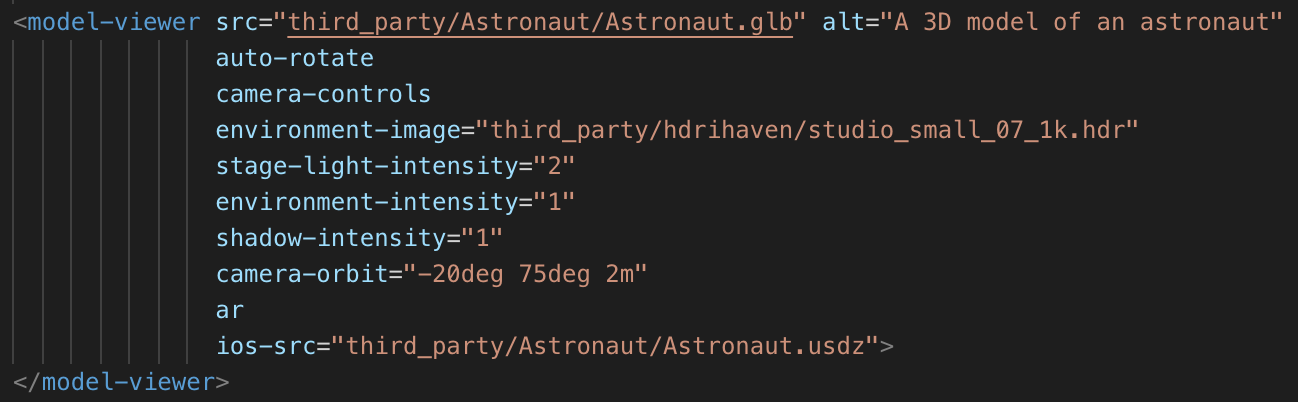
\includegraphics[width=\linewidth]{img/modelviewerhtml.png}
	\caption{De configuratie van de html-component model-viewer.}
	\label{fig:modelviewerhtml}
\end{figure}

Verder bevat de model-viewer component ook de optie om te spelen met de animaties van het 3D object, indien deze reeds gedefinieerd zijn in het model zelf. Ook kan er een hoge resolutie 360 graden achtergrondfoto ingesteld worden waardoor het lijkt dat het object zich in die omgeving bevindt. Indien dit bijvoorbeeld een foto van een hangaar zou zijn dan spiegelen alle lichtstralen vanuit die hanger op het object. 

\textbf{Concreet}

Standaard krijgen alle gebruikers het 3D-model te zien indien ze op dit moment naar een website surfen waarbij model-viewer geïmplementeerd is. In de onderstaande tabel is te zien wat er gebeurt voor de gebruikers indien er bij het model-viewer element de parameters uit de eerste kolom zijn toegevoegd

\begin{center}
	\begin{tabular}{| c | p{4.8cm} | p{4.8cm} |}
		\hline
		Ingesteld & iOS gebruikers + Chrome & iOS gebruikers + Safari \\ \hline 
		ar | ios-src & AR Quick Look opent dit object niet & AR Quick Look opent dit object wel en de gebruiker kan het plaatsen  \\ \hline
		ios-src & AR Quick Look opent dit object niet & AR Quick Look opent dit object wel en de gebruiker kan het plaatsen \\ \hline
		
	\end{tabular}
\end{center}

\begin{center}
	\begin{tabular}{| c | p{2.35cm} | p{2.35cm} | p{2.35cm} | p{2.35cm} |}
		\hline
		Ingesteld & Android vader & Android moeder & OnePlus 5 & Samsung S7 \\ \hline 
		ar & Getest op android met chrome en canary 72 maar lukt niet? & Luk niet  & Lukt wel & Lukt wel  \\ \hline
		ar | ios-src & Getest op android met chrome en canary 72 maar lukt niet? & Luk niet  & Lukt wel & Lukt wel \\ \hline
		
	\end{tabular}
\end{center}


Een puntje om hierbij op aan te merken is dat indien ontwikkelaars er voor kiezen het 3D-model te implementeren met de model-viewer component, iOS gebruikers die surfen vanop Google Chrome niet meer het model zullen kunnen zien. In tegenstelling tot Safari waar de browser het .usdz bestand herkent en daarom opent met Quick Look herkent Chrome op iOS het bestand niet en probeert het gewoon te downloaden. Eenmaal gedownload weet Chrome niet wat hij er mee moet doen en vraagt u het te openen met een ander programma. 

\section{Een derde optie}
\label{sec:een-derde-optie}

Naast de technologieën en implementeerbaarheid van de twee tech giants Google en Apple, zijn er ook nog enkele andere opties. Een daarvan is het product 8th Wall Web van het bedrijf 8th Wall. Hierbij kan u sinds 25 februari 2019 tegen een bepaalde prijs op een webplatform een Web AR applicatie ontwikkelen die u vervolgens op uw website kan plaatsen. Volgens de beschikbare demo's kan er met hun product extra interactie geïmplementeerd worden zoals het smijten van een object of het stappen door een portaal (die u naar een andere wereld brengt). Echter blijken deze AR-ervaringen niet zo soepel te zijn als de simpelere visualisatietechniek van Apple en Google. 

Vectary is een tweede voorbeeld die tot 13 maart 2019 een uitstekende online service was waarmee u 3D objecten kon maken en exporteren naar uw gewenste 3D bestandsformaat. Sinds deze specifieke dag biedt Vectary ook tegen een bepaalde prijs de mogelijkheid een 3D object of omgeving in uw website te steken.~\autocite{Vectary2019}

Het gebruik van deze 2 producten wordt in deze bachelorproef niet verder toegelicht.

%De inhoud gaat verder op de inleiding, maar zal het onderwerp van de bachelorproef *diepgaand* uitspitten. De bedoeling is dat de lezer na lezing van dit hoofdstuk helemaal op de hoogte is van de huidige stand van zaken (state-of-the-art) in het onderzoeksdomein. Iemand die niet vertrouwd is met het onderwerp, weet er nu voldoende om de rest van het verhaal te kunnen volgen, zonder dat die er nog andere informatie moet over opzoeken \autocite{Pollefliet2011}.

%Je verwijst bij elke bewering die je doet, vakterm die je introduceert, enz. naar je bronnen. In \LaTeX{} kan dat met het commando \texttt{$\backslash${textcite\{\}}} of \texttt{$\backslash${autocite\{\}}}. Als argument van het commando geef je de ``sleutel'' van een ``record'' in een bibliografische databank in het Bib\TeX{}-formaat (een tekstbestand). Als je expliciet naar de auteur verwijst in de zin, gebruik je \texttt{$\backslash${}textcite\{\}}.
%Soms wil je de auteur niet expliciet vernoemen, dan gebruik je \texttt{$\backslash${}autocite\{\}}. In de volgende paragraaf een voorbeeld van elk.

%\textcite{Knuth1998} schreef een van de standaardwerken over sorteer- en zoekalgoritmen. Experten zijn het erover eens dat cloud computing een interessante opportuniteit vormen, zowel voor gebruikers als voor dienstverleners op vlak van informatietechnologie~\autocite{Creeger2009}.

%\lipsum[7-20]
